\subsection{Cotangent spaces and the differential}

Since the tangent space is a vector space, we can do all the constructions we saw previously in the abstract vector space setting. 

\bd
Let $M$ be a manifold and $p\in M$. The \emph{cotangent space}\index{cotangent space} to $M$ at $p$ is
\bse
T^*_pM := (T_pM)^*.
\ese
\ed
Since $\dim T_pM$ is finite, we have $T_pM\cong_{\mathrm{vec}} T^*_pM$. If $\{\tvb{x}{a}{p}\}$ is the basis of $T_pM$ induced by some chart $(U,x)$, then the dual basis is denoted as $\{(\d x^a)_p\}$. We have, by definition
\bse
(\d x^a)_p \left( \tvb{x}{b}{p} \right) = \delta^a_b.
\ese

Once we have the cotangent space, we can define the tensor spaces.

\bd
Let $M$ be a manifold and $p\in M$. The \emph{tensor space $(T^r_s)_pM$} is defined as 
\bse
(T^r_s)_pM := T^r_s(T_pM) = \underbrace{T_pM\otimes\cdots\otimes T_pM}_{r \text{ copies}}\otimes\underbrace{T^*_pM\otimes\cdots\otimes T^*_pM}_{s \text{ copies}}.
\ese
\ed

\bd
Let $M$ and $N$ be manifolds and let $\phi\cl M \to N$ be smooth. The \emph{differential}\index{differential} (or \emph{derivative}) \emph{of $\phi$ at $p\in M$} is the linear map
\bi{rrCl}
\d_p \phi \cl & T_pM & \xrightarrow{\sim} & T_{\phi(p)}N\\
& X & \mapsto & \d_p\phi\,(X)
\ei
where $\d_p\phi\,(X)$ is the tangent vector to $N$ at $\phi(p)$ 
\bi{rrCl}
\d_p \phi\,(X) \cl & \mathcal{C}^\infty(N) & \xrightarrow{\sim} & \R\\
& g & \mapsto & (\d_p\phi\,(X))(g):=X(g\circ \phi).
\ei
\ed
If this definition looks confusing, it is worth it to pause and think about what it is saying. Intuitively, if $\phi$ takes us from $M$ to $N$, then $\d_p\phi$ takes us from $T_pM$ to $T_{\phi(p)}N$. The way in which it does so, is the following.
\bse
\begin{tikzcd}
M \ar[rr,"\phi"] \ar[ddrr,"g\circ\phi"'] && N \ar[dd,"g"] && \mathcal{C}^\infty(M) \ar[dd,"X"] && \mathcal{C}^\infty(N) \ar[ll,"-\circ\phi"']\ar[ddll,"\d_p\phi\,(X)"]\\
&& && &&\\
&& \R && \R&&
\end{tikzcd}
\ese
Given $X\in T_pM$, we want to construct $ \d_p\phi\,(X)\in T_{\phi(p)}N$, i.e.\ a derivation on $N$ at $f(p)$. Derivations act on functions. So, given $g\cl N\to \R$, we want to construct a real number by using $\phi$ and $X$. There is really only one way to do is. If we precompose $g$ with $\phi$, we obtain $g\circ\phi\cl M \to \R$, which is an element of $\mathcal{C}^\infty(M)$. We can then happily apply $X$ to this function to obtain a real number. You should check that $ \d_p\phi\,(X)$ is indeed a tangent vector to $N$.

\br
Note that, to be careful, we should replace $\mathcal{C}^\infty(M)$ and $\mathcal{C}^\infty(N)$ above with $\mathcal{C}^\infty(U)$ and $\mathcal{C}^\infty(V)$, where $U\se M$ and $V\se N$ are open and contain $p$ and $\phi(p)$, respectively.
\er

\be
If $M=\R^d$ and $N=\R^{d'}$, then the differential of $f\cl\R^d\to\R^{d'}$ at $p\in \R^d$
\bse
\d_pf\cl T_p \R^d\cong_\mathrm{vec}\R^d\to T_{f(p)}\R^{d'}\cong_\mathrm{vec}\R^{d'}
\ese
is none other than the Jacobian of $f$ at $p$. 
\ee

A special case of the differential is the gradient of a function in $\mathcal{C}^\infty(M)$.

\bd
Let $M$ be a manifold and let $f\cl M \to\R$ be smooth. The \emph{gradient of $f$ at $p\in M$} is the covector
\bi{rrCl}
\d_pf\cl & T_pM& \xrightarrow{\sim}& T_{f(p)} \R \cong_\mathrm{vec} \R \\
& X & \mapsto & \d_pf(X) := X(f).
\ei
In fact, we can define the \emph{gradient operator at $p\in M$} as the $\R$-linear map 
\bi{rrCl}
\d_p \cl & \mathcal{C}^\infty(U) & \xrightarrow{\sim}& T^*_pM\\
& f & \mapsto & \d_pf,
\ei
with $p\in U\se M$.
\ed

\br
Note that, by writing $\d_pf(X) := X(f)$, we have committed a slight (but nonetheless real) abuse of notation. Since $\d_pf(X)\in T_{f(p)}\R$, it takes in a function and return a real number, but $X(f)$ is already a real number! This is due to the fact that we have implicitly employed the isomorphism
\bi{rrCl}
\iota_d\cl & T_p\R^d&\to&\R^d\\
& X & \mapsto & (X(\proj_1),\ldots,X(\proj_d)),
\ei
which, when $d=1$, reads
\bi{rrCl}
\iota_1\cl & T_p\R&\to&\R\\
& X & \mapsto & X(\id_\R).
\ei
In our case, we have
\bse
\d_pf(X) := X(-\circ f) \mapsto X(\id_\R\circ f) = X(f). 
\ese
This notwithstanding, the best way to think of $\d_pf$ is as a covector, i.e.\ $\d_pf$ takes in a tangent vector $X$ and returns the real number $X(f)$, in a linear fashion.
\er

Recall that if $(U,x)$ is a chart on $M$, then the co-ordinate maps $x^a\cl U \to x(U)\se \R^{\dim M}$ are smooth functions on $U$. We can thus apply the gradient operator $\d_p$ (with $p\in U$) to each of them to obtain $(\dim M)$-many elements of $T^*_p M$.

\bp
Let $(U,x)$ be a chart on $M$, with $p\in U$. The set $\mathcal{B}=\{\d_px^a\mid 1\leq a \leq \dim M\}$ forms a basis of $T^*_p M$.
\ep

\bq
We already know that $T^*_p M = \dim M$, since it is the dual space to $T_pM$. As $|\mathcal{B}|=\dim M$ by construction, it suffices to show that it is linearly independent. Suppose that
\bse
\lambda_a \, \d_px^a = 0,
\ese
for some $\lambda_a\in \R$. Applying the left hand side to the basis element $\tvb{x}{b}{p}$ yields
\bi{rCl"s}
\lambda_a \, \d_px^a  \left( \tvb{x}{b}{p} \right)  &=& \lambda_a \tvb{x}{b}{p} (x^a ) & (definition of $\d_px^a$)\\
&=& \lambda_a \, \partial_b(x^a \circ x^{-1})(x(p)) & (definition of $\tvb{x}{b}{p}$)\\
&=& \lambda_a \, \partial_b(\proj_a)(x(p)) & \\
&=& \lambda_a \, \delta^a_b &  \\
&=& \lambda_b. & 
\ei
Therefore, $\mathcal{B}$ is linearly independent and hence a basis of $T^*_p M$. Moreover, since we have shown that
\bse
\d_px^a  \left( \tvb{x}{b}{p} \right) =\delta^a_b,
\ese
this basis is, in fact, the dual basis to $\{\tvb{x}{a}{p}\}$.
\eq

\br
Note a slight subtlety. Given a chart $(U,x)$ and the induced basis $\{\tvb{x}{a}{p}\}$ of $T_pM$, the dual basis to $\{\tvb{x}{a}{p}\}$ exists simply by virtue of $T^*_pM$ being the dual space to $T_pM$. What we have shown above is that the elements of this dual basis are given explicitly by the gradients of the co-ordinate maps of $(U,x)$. In our notation, we have
\bse
(\d x^a)_p = \d_p x^a , \qquad 1\leq a \leq \dim M.
\ese
\er

\subsection{Push-forward and pull-back}

The push-forward of a smooth map $\phi\cl M\to N$ at $p\in M$ is just another name for the differential of $\phi$ at $p$. We give the definition again in order to establish the new notation.

\bd
Let $\phi\cl M \to N$ be a smooth map between smooth manifolds. The \emph{push-forward}\index{push-forward} of $\phi$ at $p\in M$ is the linear map:
\bi{rrCl}
(\phi_*)_p \cl & T_pM & \xrightarrow{\sim} & T_{\phi(p)}N\\
& X & \mapsto & (\phi_*)_p(X) := X(-\circ \phi).
\ei
\ed

If $\gamma\cl\R\to M$ is a smooth curve on $M$ and $\phi\cl M\to N$ is smooth, then $\phi\circ\gamma\cl \R \to N$ is a smooth curve on $N$. 

\bp
Let $\phi\cl M\to N$ be smooth. The tangent vector $X_{\gamma,p}\in T_pM$ is pushed forward to the tangent vector $X_{\phi\circ\gamma,\phi(p)}\in T_{\phi(p)}N$, i.e.\
\bse
(\phi_*)_p(X_{\gamma,p}) = X_{\phi\circ\gamma,\phi(p)}.
\ese
\ep

\bq
Let $f\in \mathcal{C}^\infty(V)$, with $(V,x)$ a chart on $N$ and $\phi(p)\in V$. By applying the definitions, we have
\bi{rCl"s}
(\phi_*)_p(X_{\gamma,p}) (f)& = & (X_{\gamma,p}) (f\circ\phi) & (definition of $(\phi_*)_p$)\\
& = &  ((f\circ\phi)\circ \gamma)'(0) & (definition of $X_{\gamma,p}$)\\
& = &  (f\circ(\phi\circ \gamma))'(0) & (associativity of $\circ$)\\
& = &  X_{\phi\circ\gamma,\phi(p)}(f) & (definition of $X_{\phi\circ\gamma,\phi(p)}$)
\ei
Since $f$ was arbitrary, we have $(\phi_*)_p(X_{\gamma,p}) = X_{\phi\circ\gamma,\phi(p)}$.
\eq

Related to the push-forward, there is the notion of pull-back of a smooth map.

\bd
Let $\phi\cl M \to N$ be a smooth map between smooth manifolds. The \emph{pull-back}\index{pull-back} of $\phi$ at $p\in M$ is the linear map:
\bi{rrCl}
(\phi^*)_p \cl & T^*_{\phi(p)}N & \xrightarrow{\sim} & T^*_pM\\
& \omega & \mapsto & (\phi^*)_p(\omega),
\ei
where $(\phi^*)_p(\omega)$ is defined as
\bi{rrCl}
(\phi^*)_p(\omega) \cl & T_pM & \xrightarrow{\sim} & \R\\
& X & \mapsto & \omega((\phi_*)_p(X)),
\ei
\ed
In words, if $\omega$ is a covector on $N$, its pull-back $(\phi^*)_p(\omega)$ is a covector on $M$. It acts on tangent vectors on $M$ by first pushing them forward to tangent vectors on $N$, and then applying $\omega$ to them to produce a real number.

\br
If you don't see it immediately, then you should spend some time proving that all the maps that we have defined so far and \emph{claimed} to be linear are, in fact, linear.
\er

\br
We have seen that, given a smooth $\phi\cl M\to N$, we can push a vector $X\in T_pM$ forward to a vector $(\phi_*)_p(X)\in T_{\phi(p)}N$, and pull a covector $\omega \in T^*_{\phi(p)}N$ back to a covector $(\phi^*)_p(\omega)\in T_p^*M$.

\bse
\begin{tikzcd}
\mathcal{C}^\infty(M) \ar[dd,"X"] && \mathcal{C}^\infty(N) \ar[ll,"-\circ\phi"']\ar[ddll,"(\phi_*)_p(X)"]   && T_pM \ar[rr,"(\phi_*)_p"] \ar[ddrr,"(\phi^*)_p(\omega)"'] && T_{\phi(p)}N \ar[dd,"\omega"]\\
&& && &&\\
\R&& && && \R
\end{tikzcd}
\ese

However, if $\phi\cl M\to N$ is a diffeomorphism, then we can also pull a vector $Y\in T_{\phi(p)}N$ back to a vector $(\phi^*)_p(Y)\in T_pM$, and push a covector $\eta \in T^*_pM$ forward to a covector $(\phi_*)_p(\eta)\in T_{\phi(p)}^*N$, by using $\phi^{-1}$ as follows:
\bi{rCl}
(\phi^*)_p(Y) & := & ((\phi^{-1})_*)_{\phi(p)}(Y)\\
(\phi_*)_p(\eta) & := & (({\phi^{-1}})^*)_{\phi(p)}(\eta).
\ei

\bse
\begin{tikzcd}
\mathcal{C}^\infty(M) \ar[rr,"-\circ\phi^{-1}"] \ar[ddrr,"(\phi^*)_p(Y)"'] && \mathcal{C}^\infty(N) \ar[dd,"Y"]    && T_pM \ar[dd,"\eta"']   &&& T_{\phi(p)}N \ar[lll,"((\phi^{-1})_*)_{\phi(p)}"'] \ar[ddlll,"(\phi_*)_p(\eta)"] \\
&& && &&\\
&& \R && \R && 
\end{tikzcd}
\ese
This is only possible if $\phi$ is a diffeomorphism. In general, you should keep in mind that
\begin{center}
\emph{Vectors are pushed forward,\\ covectors are pulled back.}
\end{center}
\er

\br
Given a smooth map $\phi\cl M \to N$, if $f\in \mathcal{C}^\infty (N)$, then $f\circ \phi$ is often called the pull-back of $f$ along $\phi$. Similarly, if $\gamma$ is a curve on $M$, then $\phi \circ \gamma$ is called the push-forward of $\gamma$ along $\phi$. For example, we can say that 
\begin{itemize}
\item the push-forward of a tangent vector acting on a function is the tangent vector acting on the pull-back of the function;
\item the push-forward of a tangent vector to a curve is the tangent vector to the push-forward of the curve.
\end{itemize}
\er

\subsection{Immersions and embeddings}

We will now consider the question of under which circumstances a smooth manifold can ``sit'' in $\R^d$, for some $d\in \N$. There are, in fact, two notions of sitting inside another manifold, called immersion and embedding.

\bd
A smooth map $\phi\cl M \to N$ is said to be an \emph{immersion}\index{immersion} of $M$ into $N$ if the derivative
\bse
\d_p\phi \equiv (\phi_*)_p \cl T_pM\xrightarrow{\sim}T_{\phi(p)}N
\ese
is injective, for all $p\in M$. The manifold $M$ is said to be an \emph{immersed submanifold} of $N$.
\ed

% \be
% \ben[label=\alph*)]
% \item $S^1\to \R^2$ 
% \begin{center}
% \begin{tikzpicture}[scale=0.6]
% \node (v9) at (-4,1) {};
% \node (v10) at (0,1) {};
% \node (v11) at (-3,-2) {};
% \node (v12) at (-1,-2) {};
% \node (v2) at (2.5,2.5) {};
% \node (v1) at (2.5,-4) {};
% \node (v3) at (2,-3.5) {};
% \node (v4) at (9,-3.5) {};
% \node (v5) at (-4,-2.8) {};
% \node (v6) at (-3.5,-1.3) {};
% \node (v7) at (-0.5,-2.8) {};
% \node (v8) at (0,-1.3) {};
% \draw (-8.5,-1) ellipse (2 and 2);
% \draw [arrows={-angle 90}] (v1) edge (v2);
% \draw [arrows={-angle 90}] (v3) edge (v4);
% \draw [-triangle 60,blue] (v5) edge (v6);
% \draw [-triangle 60,red] (v7) edge (v8);
% \draw [arrows={-angle 90}] (v9) edge (v10);
% \draw [arrows={-angle 90}] (v11) edge (v12);
% \draw  plot[smooth cycle, tension=.7] coordinates {(3.5,-1) (3.5,-2) (4,-2.5) (5,-2.5) (5.5,-2) (5.5,-1.5) (6.5,-1) (7.5,-1.5) (8.5,-2) (9,-1) (9,0) (8,0.5) (7,0.5) (6,0.5) (5.5,0) (5,0) (4,-0.5)};
% \node (v13) at (4.5,6) {};
% \node (v14) at (9,0) {};
% \node (v17) at (13.5,-6) {};
% \node (v19) at (8,1.3) {};
% \node (v20) at (10,-1.4) {};
% \node (v16) at (-9,1.74) {};
% \node (v15) at (-7.5,0.74) {};
% \node (v18) at (-6,-0.26) {};
% \draw [-triangle 60,blue] (v15) edge (v18);
% \draw [-triangle 60,blue] (v15) edge (v16);
% \node at (-2,1.5) {$\phi$};
% \node at (-2,-1.5) {$\phi_*$};
% \node at (3.5,2) {$\R^2$};
% \node at (-11,0.5) {$S^1$};
% \node at (3.75,0.3) {$\phi(S^1)$};
% \draw [-triangle 60,red] (v14) edge (v19);
% \draw [-triangle 60,red] (v14) edge (v20);
% \end{tikzpicture}
% \end{center}
% \item 
% \een
% \ee

From the theory of linear algebra, we immediately deduce that, for $\phi\cl M\to N$ to be an immersion, we must have $\dim M \leq \dim N$. A closely related notion is that of a \emph{submersion}, where we require each $(\phi_*)_p$ to be surjective, and thus we must have $\dim M \geq \dim N$. However, we will not need this here. 

\be
Consider the map $\phi\cl S^1\to \R^2$ whose image is reproduced below.

\begin{center}
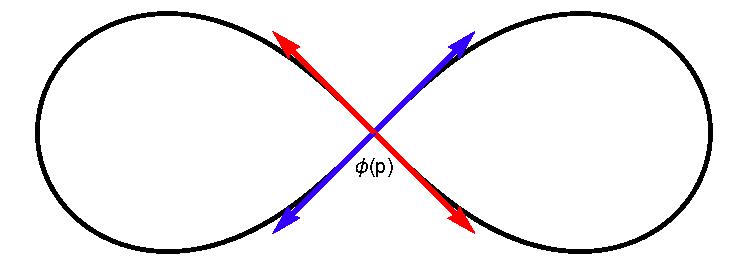
\includegraphics[scale=0.8]{graphics/immers}
\end{center}
\ee
The map $\phi$ is not injective, i.e.\ there are $p,q\in S^1$, with $p\neq q$ and $\phi(p)=\phi(q)$. Of course, this means that $T_{\phi(p)}\R^2=T_{\phi(q)}\R^2$. However, the maps $(\phi_*)_p$ and $(\phi_*)_q$ are both injective, with their images being represented by the blue and red arrows, respectively. Hence, the map $\phi$ is immersion.

\bd
A smooth map $\phi\cl M \to N$ is said to be a \emph{(smooth) embedding}\index{embedding} of $M$ into $N$ if
\begin{itemize}
\item $\phi\cl M\to N$ is an immersion;
\item $M \cong_{\mathrm{top}}\phi(M)\se N$, where $\phi(M)$ carries the subset topology inherited from $N$.
\end{itemize}
The manifold $M$ is said to be an \emph{embedded submanifold} of $N$.
\ed

\br
If a continuous map between topological spaces satisfies the second condition above, then it is called a \emph{topological embedding}. Therefore, a smooth embedding is a topological embedding which is also an immersion (as opposed to simply being a smooth topological embedding).
\er

In the early days of differential geometry there were two approaches to study manifolds. One was the extrinsic view, within which manifolds are defined as special subsets of $\R^d$, and the other was the intrinsic view, which is the view that we have adopted here.

Whitney's theorem, which we will state without proof, states that these two approaches are, in fact, equivalent.

\begin{theorem}[Whitney]
Any smooth manifold $M$ can be
\begin{itemize}
\item embedded in $\R^{2\dim M}$;
\item immersed in $\R^{2\dim M-1}$.
\end{itemize}
\end{theorem}

\be
The Klein bottle can be embedded in $\R^4$ but not in $\R^3$. It can, however, be immersed in $\R^3$.
\ee

What we have presented above is referred to as the \emph{strong} version of Whitney's theorem. There is a weak version as well, but there are also even stronger versions of this result, such as the following.

\begin{theorem}
Any smooth manifold can be immersed in $\R^{2\dim M-a(\dim M)}$, where $a(n)$ is the number of $1$s in a binary expansion of $n\in \N$.
\end{theorem}

\be
If $\dim M = 3$, then as 
\bse
3_{10}=(1\times 2^1+1\times 2^0)_{10}=11_2,
\ese
we have $a(\dim M)=2$, and thus every $3$-dimensional manifold can be immersed into $\R^4$. Note that even the strong version of Whitney's theorem only tells us that we can immerse $M$ into $\R^5$.
\ee

\subsection{The tangent bundle}

We would like to define a vector field on a manifold $M$ as a ``smooth'' map that assigns to each $p\in M$ a tangent vector in $T_pM$. However, since this would then be a ``map'' to a different space at each point, it is unclear how to define its smoothness. 

The simplest solution is to merge all the tangent spaces into a unique set and equip it with a smooth structure, so that we can then define a vector field as a smooth map between smooth manifolds.

\bd
Given a smooth manifold $M$, the \emph{tangent bundle} of $M$ is the disjoint union of all the tangent spaces to $M$, i.e.\
\bse
TM :=\coprod_{p\in M}T_pM,
\ese
equipped with the canonical projection map
\bi{rrCl}
\pi \cl & TM & \to & M\\
& X & \mapsto & p,
\ei
where $p$ is the unique $p\in M$ such that $X\in T_pM$.
\ed

We now need to equip $TM$ with the structure of a smooth manifold. We can achieve this by constructing a smooth atlas for $TM$ from a smooth atlas on $M$, as follows.

Let $\mathscr{A}_M$ be a smooth atlas on $M$ and let $(U,x)\in \mathscr{A}_M$. If $X\in \preim_\pi(U)\se TM$, then $X\in T_{\pi(X)}M$, by definition of $\pi$. Moreover, since $\pi(X)\in U$, we can expand $X$ in terms of the basis induced by the chart $(U,x)$:
\bse
X = X^a \tvb{x}{a}{\pi(X)},
\ese
where $X^1,\ldots,X^{\dim M}\in \R$. We can then define the map
\bi{rrCl}
\xi \cl & \preim_\pi(U) & \to & x(U) \times \R^{\dim M} \cong_{\mathrm{set}}\R^{2\dim M}\\
& X & \mapsto & (x(\pi(X)),X^1,\ldots,X^{\dim M}).
\ei
Assuming that $TM$ is equipped with a suitable topology, for instance the initial topology (i.e.\ the coarsest topology on $TM$ that makes $\pi$ continuous), we claim that the pair $(\preim_\pi(U),\xi)$ is a chart on $TM$ and 
\bse
\mathscr{A}_{TM} := \{(\preim_\pi(U),\xi)\mid (U,x) \in \mathscr{A}_M\}
\ese
is a smooth atlas on $TM$. Note that, from its definition, it is clear that $\xi$ is a bijection. We will not show that $(\preim_\pi(U),\xi)$ is a chart here, but we will show that $\mathscr{A}_{TM}$ is a smooth atlas.

\bp
Any two charts $(\preim_\pi(U),\xi), (\preim_\pi(\widetilde U),\widetilde \xi)\in\mathscr{A}_{TM}$ are $\mathcal{C}^\infty$-compatible.
\ep

\bq
Let $(U,x)$ and $(\widetilde U,\widetilde x)$ be the two charts on $M$ giving rise to $(\preim_\pi(U),\xi)$ and $(\preim_\pi(\widetilde U),\widetilde \xi)$, respectively. We need to show that the map
\bse
\widetilde \xi \circ \xi^{-1} \cl x(U\cap \widetilde U)\times \R^{\dim M} \to \widetilde x(U\cap\widetilde U)\times \R^{\dim M}
\ese
is smooth, as a map between open subsets of $\R^{2\dim M}$. Recall that such a map is smooth if, and only if, it is smooth componentwise. On the first $\dim M$ components, $\widetilde \xi \circ \xi^{-1} $ acts as
\bi{rrCl}
\widetilde x \circ x^{-1} \cl & x(U\cap \widetilde U)& \to &\widetilde x(U\cap\widetilde U)\\
& x(p) & \mapsto & \widetilde x(p),
\ei
while on the remaining $\dim M$ components it acts as the change of vector components we met previously, i.e.\
\bse
X^a \mapsto \widetilde X^a = \partial_b(y^a\circ x^{-1})(x(p))\, X^b.
\ese
Hence, we have
\bi{rrCl}
\widetilde \xi \circ \xi^{-1} \cl & x(U\cap \widetilde U)\times \R^{\dim M} &\to &\widetilde x(U\cap\widetilde U)\times \R^{\dim M}\\
& (x(\pi(X)),X^1,\ldots,X^{\dim M})& \mapsto & (\widetilde x(\pi(X)),\widetilde X^1,\ldots,\widetilde X^{\dim M}),
\ei
which is smooth in each component, and hence smooth.
\eq
The tangent bundle of a smooth manifold $M$ is therefore itself a smooth manifold of dimension $2\dim M$, and the projection $\pi\cl TM\to M$ is smooth with respect to this structure. 

Similarly, one can construct the \emph{cotangent bundle} $T^*M$ to $M$ by defining
\bse
T^*M := \coprod_{p\in M} T^*_pM
\ese
and going through the above again, using the dual basis $\{(\d x^a)_p\}$ instead of $\{\tvb{x}{a}{p}\}$.






















